\chapter{Présentation de l'interface:}
\section{Au premier lancement}
La première fois que vous lancez XLogo (ou si vous avez effacé le fichier \texttt{.xlogo} - Voir section \ref{fichier_perso}), une boîte de dialogue apparaîtra pour vous permettre de choisir la langue utilisée.
\begin{center}
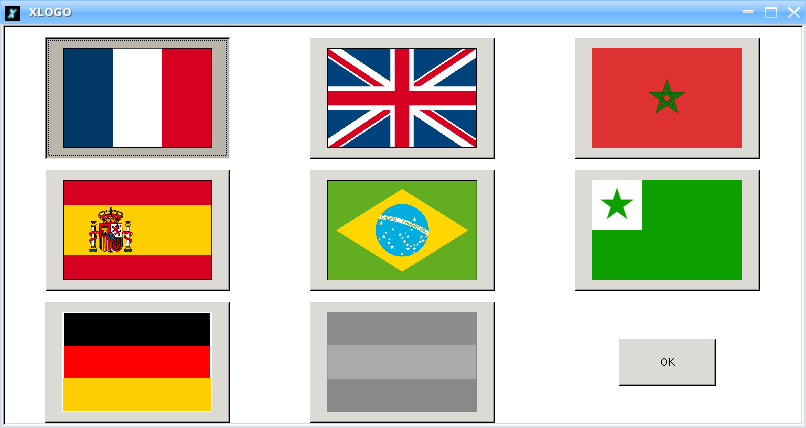
\includegraphics[scale=0.2]{images/CaptureLangue.png} 
\end{center}
Ce choix n'est pas définitif bien sûr, il peut être corrigé ensuite à l'aide de la boîte de dialogue de Préférences. (Voir section \ref{onglet_general})
\section{Fenêtre principale}
\begin{center}
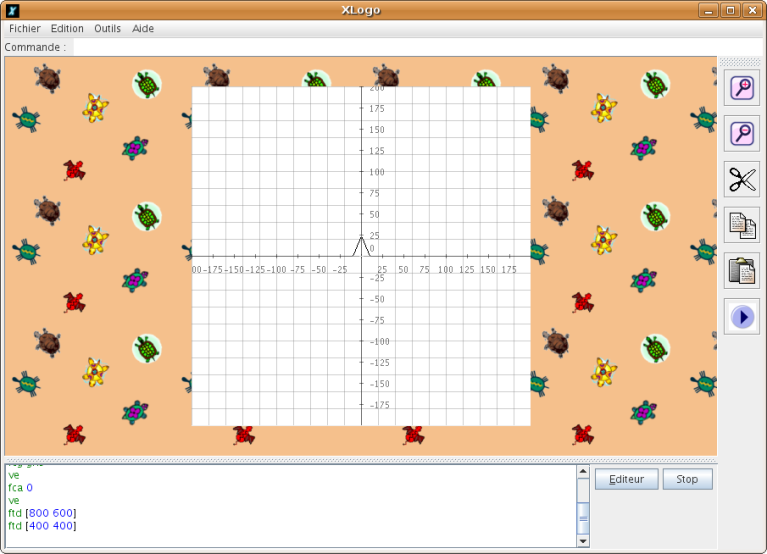
\includegraphics[scale=0.45]{images/Capture.png} 
\end{center}
\begin{itemize}
\item En haut, les traditionnels menus \begin{large}  \textbf{Fichier, Edition, Outils et
Aide}   \end{large}
\item Juste en dessous, \textbf{\begin{large}la ligne de commande\end{large}} qui permet de saisir les instructions
logo.
\item Au centre, \begin{large}\textbf{la zone de dessin}\end{large}.
\item A la droite de la zone de dessin, \textbf{\begin{large}une barre d'outils\end{large}} vous permet de réaliser divers actions:
\begin{itemize}
\item Zoom avant/arrière.
\item Diverses fonctionnalités d'édition (couper/copier/coller).
\item Le bouton \og Lecture\fg\ permet de lancer la commande principale définie dans l'éditeur.
\end{itemize}
\item En bas, \begin{large}\textbf{la zone \og historique \fg}\end{large} \ qui rappelle toutes les dernières commandes tapées et les réponses associées. Pour rappeler rapidement une instruction déjà tapée, il y a deux solutions: ou bien vous cliquez sur l'ancienne instruction dans l'historique, ou bien vous appuyez plusieurs fois sur la flèche du haut jusqu'à ce que l'instruction désirée apparaisse. Les deux flèches haut et bas permettent en fait de se déplacer dans toute l'historique des commandes tapées précédemment (Très pratique).
\item A la droite de l'historique, deux boutons: \begin{large}\textbf{STOP et EDITEUR} \end{large}.
\begin{itemize}
 \item Le bouton STOP interrompt toute exécution en cours. 
\item Le bouton EDITEUR permet d'ouvrir l'éditeur de procédures.
\end{itemize}
\end{itemize}
\section{L'éditeur de procédures}
\begin{center}
 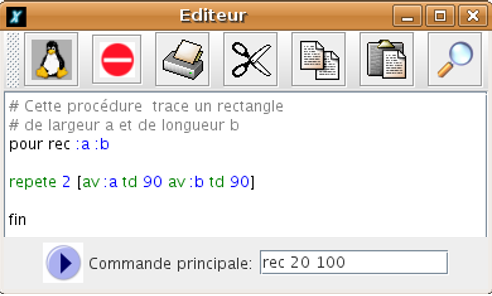
\includegraphics[scale=0.4]{images/CaptureEditeur.png}
\end{center}
Pour ouvrir l'éditeur, trois possibilités:
\begin{itemize}
\item Taper \texttt{ed} dans la ligne de commandes. L'éditeur s'ouvrira alors avec toutes les procédures déjà définies. Si vous ne souhaitez éditer que certaines procédures particulières, taper alors:\\ \texttt{ed [procedure\_1 procedure\_2 ...]}
\item Appuyer sur le bouton Editeur de la fenêtre principale.
\item Utiliser le raccourci clavier Alt+E
\end{itemize} 
\vspace{0.5cm}
Voici les différents boutons que vous trouverez dans l'éditeur:\\

\begin{longtable}{cm{12cm}}
\includegraphics*[scale=1]{images/tortue.png} & Sauve les modifications apportés au contenu de l'éditeur puis ferme celui-ci. C'est sur ce bouton qu'il faut appuyer à chaque fois que vous voulez enregistrer les nouvelles procédures tapées. Si vous le préférez, vous pouvez utiliser le raccourci clavier ALT+Q.\\
\includegraphics*[scale=1]{images/quit.png} & Quitte l'éditeur en n'enregistrant aucune des modifications apportées à celui-ci. On peut également utiliser le raccourci ALT+C.\\
\includegraphics*[scale=1]{images/fileprint.png} & Imprime le contenu de l'éditeur.\\
\includegraphics*[scale=1]{images/editcopy.png} & Copie le texte sélectionné dans le presse-papiers\\
\includegraphics*[scale=1]{images/editcut.png} & Coupe le texte sélectionné dans le presse-papiers\\
\includegraphics*[scale=1]{images/editpaste.png} & Colle le texte sélectionné dans le presse-papiers\\
\includegraphics*[scale=1]{images/chercher.png} & Ouvre une boîte de dialogue permettant de chercher ou de remplacer du texte dans l'éditeur.\\
\end{longtable} 
\begin{center}
 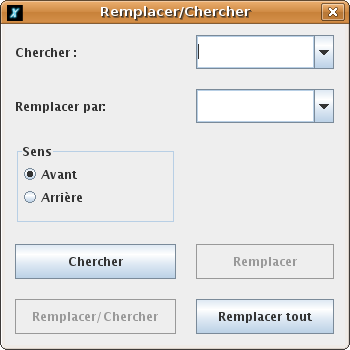
\includegraphics[scale=0.4]{images/CaptureChercher.png}
\end{center}
\vspace{0.5cm}

\includegraphics{images/play.png}
Tout en bas de l'éditeur, un champ texte permet de définir une commande principale. Celle-ci représente la commande générale qui permet de lancer un programme. Elle est accessible via le bouton \og lecture\fg\ de la barre d'outils de la fenêtre principale. Lorsqu'on sauve le contenu de l'éditeur dans un fichier au format \texttt{.lgo}, cette commande est également enregistrée \\ \\
\textbf{\begin{Large}IMPORTANT\end{Large}}: \\
\begin{itemize}
\item Cela ne sert à rien d'appuyer sur la croix en haut à droite pour fermer la fenêtre! Seuls les deux premiers boutons vous permettent de quitter l'éditeur.
\item Pour effacer une ou plusieurs procédures indésirables, utiliser la primitive \texttt{efp, effaceprocedure} ou alors utiliser dans la barre de menus \textbf{Outils - Gestionnaire de procédures}.
\end{itemize} 
\section{Quitter}
Pour quitter XLogo, dans la barre de menu, \textbf{Fichier - Quitter} ou alors cliquer sur la croix de fermeture de la fenêtre. Une boîte de dialogue de confirmation apparaît à ce moment.
\begin{center}
 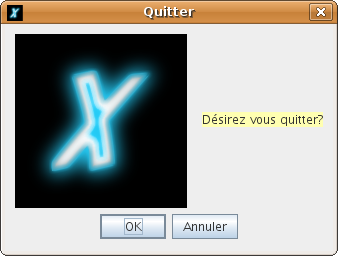
\includegraphics[scale=0.4]{images/CaptureQuitter.png}
\end{center}
\chapter{Options des menus:}
\section{Menu \og Fichier \fg}
\begin{itemize}
\item \textbf{Fichier$\to$Nouveau}: Détruit l'ensemble des procédures et variables définies pour créer ainsi un nouvel espace de travail.\\
\item \textbf{Fichier$\to$Ouvrir}: ouvre un fichier logo précédemment enregistré.
\begin{center}
 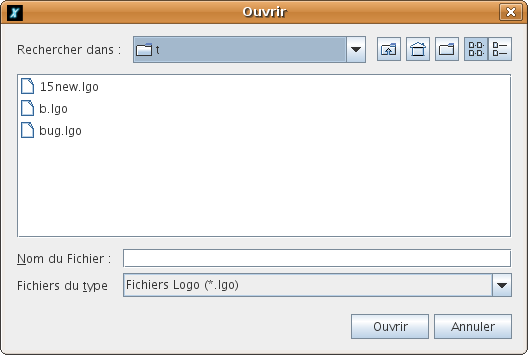
\includegraphics[scale=0.4]{images/CaptureOuvrir.png}
\end{center}
\vspace{0.25cm}
\item \textbf{Fichier$\to$Enregistrer sous ...}: enregistre les procédures en cours
sous un nom précis.
\begin{center}
 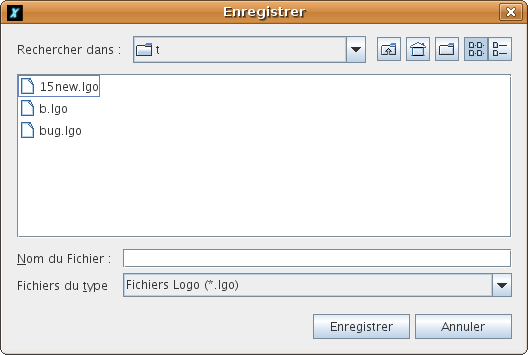
\includegraphics[scale=0.4]{images/CaptureEnregistrer.png}
\end{center}
\vspace{0.25cm}
\item \textbf{Fichier$\to$Enregistrer}: enregistre les procédures dans le fichier actuellement utilisé.\\
\item \textbf{Fichier$\to$Capturer l'image$\to$Enregistrer l'image sous...} : permet
d'enregistrer l'image sous le format jpg ou png. Si vous souhaitez
sélectionner seulement une partie de l'image, vous avez la possibilité
de définir un rectangle de sélection en faisant glisser la souris sur la zone de dessin.\\
\item \textbf{Fichier$\to$Capturer l'image$\to$Imprimer l'image} : permet d'imprimer
l'image. De même que précédemment, vous pouvez sélectionner
une zone précise à imprimer.\\
\item \textbf{Fichier$\to$Capturer l'image$\to$Copier l'image dans le presse-papier}: Permet d'envoyer l'image dans le presse-papier système. De même que pour l'impression et l'enregistrement, vous pouvez ne sélectionner qu'une zone de l'image. Cette fonctionnalité fonctionne très bien sous les environnements de type Windows. En revanche, elle ne marche pas sous Linux (Le presse-papier n'a pas le même type de fonctionnement). Non testé sous Mac.\\
\item \textbf{Fichier$\to$Zone de texte$\to$Enregistrer au format RTF}: Permet d'enregistrer la zone d'historique au format RTF (conserve les couleurs et le formatage des caractères).\\
\item \textbf{Fichier$\to$Quitter}: quitte l'application XLOGO.\\
\end{itemize}

\section{Menu \og Edition \fg}
\begin{itemize}
\item \textbf{Edition$\to$Copier}: copie le texte sélectionné dans le presse-papiers.\\
\item \textbf{Edition$\to$Couper}: coupe le texte sélectionné dans le presse-papiers.\\
\item \textbf{Edition$\to$Coller}: colle le texte contenu dans le presse-papiers dans
la ligne de commande.\\
\item \textbf{Edition$\to$Sélectionner tout}: Sélectionne l'ensemble du texte de la zone de commande.
\end{itemize}

\section{Menu \og Outils \fg}
\begin{itemize}
\item \textbf{Outils$\to$Choisir la couleur du crayon}: permet de choisir la couleur
avec laquelle écrit la tortue à l'aide d'une palette de couleurs.\\
\begin{center}
 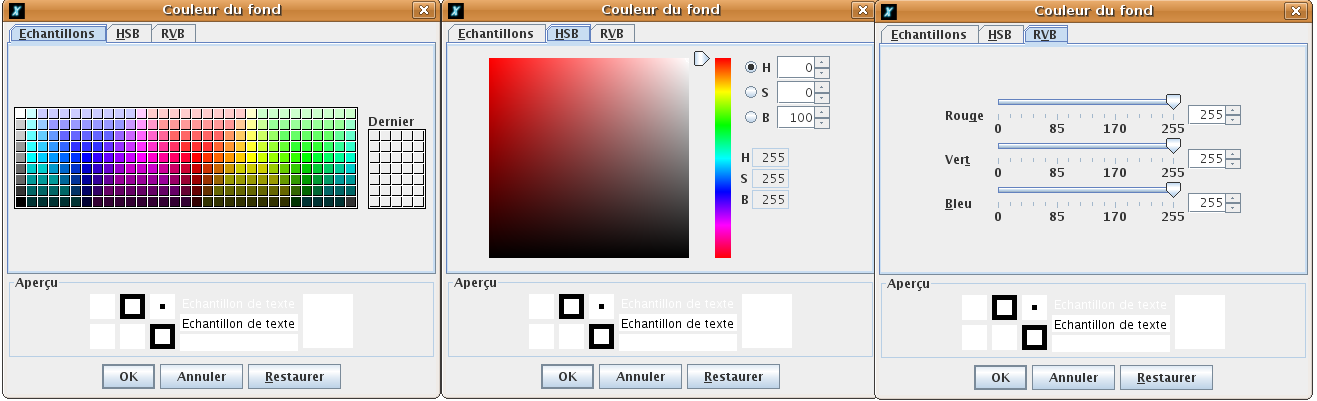
\includegraphics[scale=0.3]{images/CaptureCouleur.png}
\end{center}
\vspace{0.25cm}
Disponible également avec la primitive \texttt{fcc} (Voir annexe \ref{fcc}).\\
\item \textbf{Outils$\to$Choisir la couleur du fond}: même chose avec le fond d'écran.
Disponible avec la primitive \texttt{fcfg}. (Voir annexe \ref{fcfg}).\\
\item \textbf{Outils$\to$Définir les fichiers de démarrage}: permet de définir des chemins vers des fichiers dit \og de démarrage \fg. Toutes les procédures contenues dans ces fichiers au format *.lgo deviendront alors des \og pseudo-primitives \fg \ du langage XLogo. Elles ne sont pas éditables ni modifiables par l'utilisateur. Vous pouvez ainsi définir des primitives personnalisées. Vous pouvez de plus lui donner une commande (en logo) à effectuer au démarrage de XLogo. Vous avez ainsi la possibilité de lancer un programme que vous avez conçu dès l'ouverture de XLogo.\\
\begin{center}
 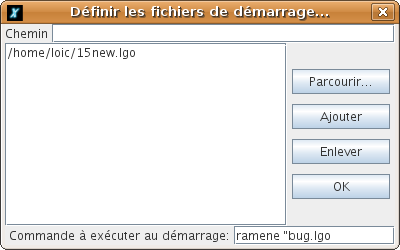
\includegraphics[scale=0.4]{images/CaptureDemarrage.png}
\end{center}
\vspace{0.25cm}
\item \textbf{Outils$\to$Traduire des procédures}: Ouvre une boîte de dialogue qui permet de traduire des commandes XLogo dans une langue désirée. (Très utile en particulier lorsqu'on récupère des sources Logo en anglais sur internet pour les remettre en français)\\
\begin{center}
 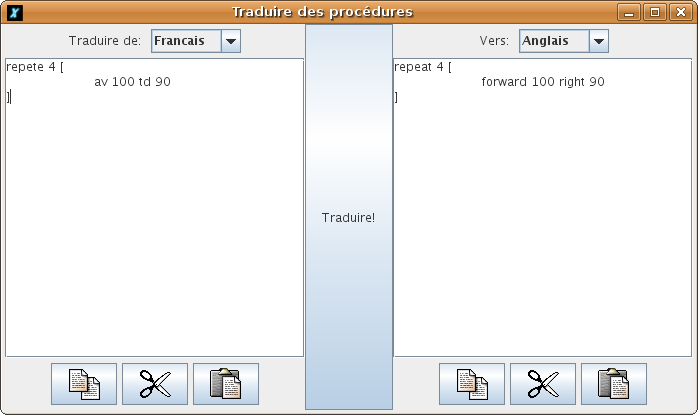
\includegraphics[scale=0.4]{images/CaptureTraduire.png}
\end{center}
\vspace{0.25cm}
\item \textbf{Outils$\to$Gestionnaire de procédures}: Ouvre une boîte de dialogue permettant d'effacer des procédures. Elle permet également de changer l'ordre d'apparition des procédures dans l'éditeur.\\
\begin{center}
 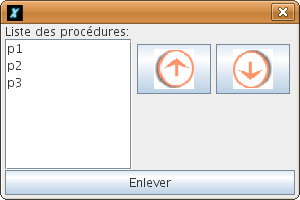
\includegraphics[scale=0.4]{images/CaptureProcedure.png}
\end{center}
\vspace{0.25cm}
\item \textbf{Options$\to$Préférences}: Ouvre une boîte de dialogue dans laquelle vous pouvez configurer plusieurs choses:
\begin{itemize} 
 	\item \textbf{Onglet général:} \label{onglet_general}
	\begin{itemize}
 	\item \textbf{Langue}: permet de choisir entre le français, l'anglais, l'espagnol, le portugais, l'arabe, l'allemand et l'espéranto. Attention, les primitives changent d'une langue à, l'autre.\\
	\item \textbf{Aspect:} permet de définir le \og look \fg \ de la fenêtre XLogo. Soit style natif, style Java (Métal) ou style Motif\\
	\item \textbf{Choisir la vitesse de défilement}. Si vous souhaitez voir tous les déplacement de la tortue, vous pouvez la ralentir à l'aide
de la barre prévue à cet effet.
	\begin{center}
 		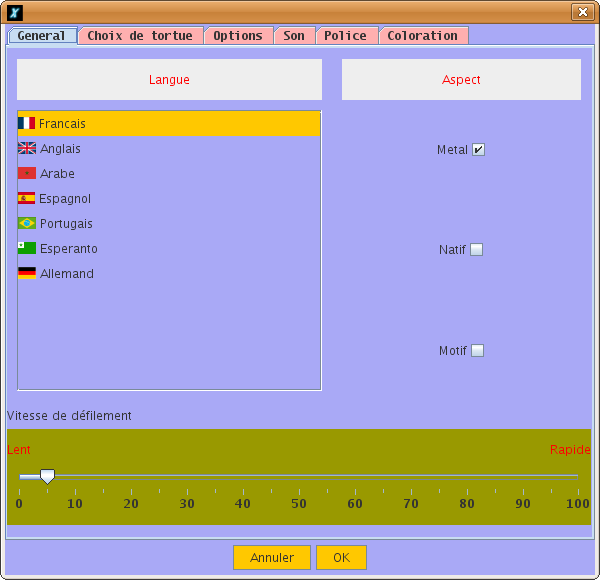
\includegraphics[scale=0.3]{images/CapturePref1.png}\\
\vspace*{1cm}
 		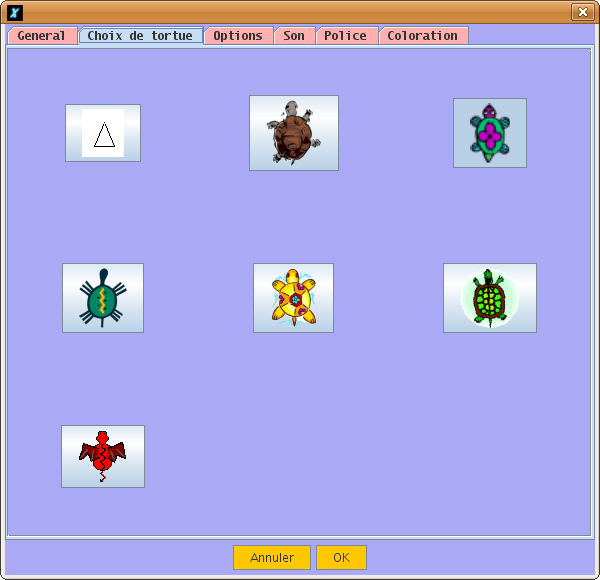
\includegraphics[scale=0.3]{images/CapturePref2.png}
	\end{center}
	\vspace{0.25cm}
	\end{itemize}
	\item \textbf{Onglet Choix de la tortue}: vous pouvez choisir votre tortue préférée.\\
	\begin{center}
 		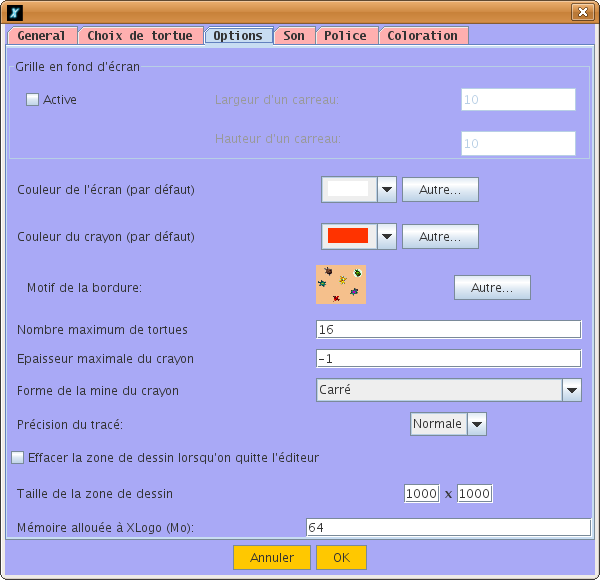
\includegraphics[scale=0.4]{images/CapturePref3.png}
	\end{center}
	\item \textbf{Onglet Options}: Plusieurs choses peuvent être fixées. 
	\begin{itemize}
		\item \textbf{Grille:} vous pouvez choisir de tracer une grille en fond d'écran. Il est possible de choisir la largeur et la hauteur d'un carreau de la grille ainsi que sa couleur.
		\item \textbf{Axes:} vous pouvez choisir de tracer l'axe vertical ou l'axe vertical en fond d'écran. Vous pouvez définir la distance entre deux graduations ainsi que la couleur de chaque axe.
		\item \textbf{Couleur de fond d'écran}: Possibilité de définir une couleur de fond d'écran par défaut.
		\item \textbf{Couleur de crayon}: Possibilité de définir une couleur de crayon par défaut.
		\item \textbf{Motif de bordure}: Possibilité de définir un motif précis pour la bordure encadrant la zone de dessin (soit sous forme d'une image soit sous forme d'une couleur unie.)
	\begin{center}
 		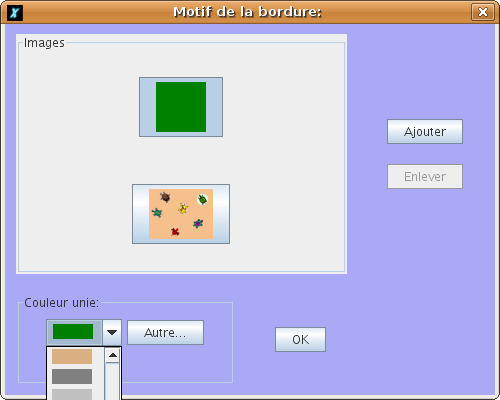
\includegraphics[scale=0.4]{images/CaptureBordure.png}
	\end{center}
		\item \textbf{Epaisseur du crayon}: On peut fixer une taille limite à l'épaisseur du crayon. Si l'on ne veut pas utiliser cette limitation, mettre le nombre -1 dans la zone de texte associée.
		\item \textbf{Forme du crayon}: Ensuite, on peut choisir la forme du crayon de la tortue, on ne se rend compte du choix de cette option que lorsque l'on choisit une épaisseur de crayon supérieure à 1.
		\item \textbf{Nombre maximal de tortues}: On peut également fixer le nombre de tortues maximum en mode multitortues. (Par défaut 16)
		\item \textbf{Précision du tracé}: Vous pouvez choisir la qualité du tracé. En haute qualité, vous n'aurez plus d'effet de crénelage des lignes. En revanche, bien repérer qu'en augmentant la qualité, vous perdrez en rapidité d'exécution.
		\item \textbf{Effacer la zone de dessin en sortie d'éditeur}: On peut choisir d'effacer automatiquement la zone de dessin lorsqu'on sort de l'éditeur.
		\item \textbf{Effacer les variables en sortie d'éditeur}: Certains utilisateurs apprécient qu'à chaque changement dans l'éditeur, les variables globales soient automatiquement détruites. C'est possible en activant cette option.
		\item \textbf{Taille de la zone de dessin}: Vous pouvez choisir une taille personnalisée pour la zone de tracé. Par défaut XLogo se lance avec une zone de 1000 pixels sur 1000 pixels. \textcolor{red} {Attention}, lorsque vous agrandissez l'image, il peut-être nécessaire d'augmenter la taille mémoire attribuée à XLogo. Un message d'erreur vous en avertira.
		\item \textbf{Mémoire allouée à XLogo}: Vous pouvez par conséquent également changer la valeur correspondant à l'espace mémoire alloué à XLogo. Par défaut, cette valeur est fixée à 64 Mo. Il se peut que vous soyez obligé de l'augmenter si vous souhaitez travailler sur une zone de dessin plus grande. Lorsqu'on modifie ce paramètre, le changement n'est effectif qu'après redémarrage de XLogo. \textcolor{red} {Attention, n'augmentez pas abusivement sans raison cette valeur, cela peut considérablement ralentir votre système.}
		\item \textbf{Numéro du port TCP:} Permet de choisir une valeur particulière pour le port utilisé lors des communications réseau. Voir p.\pageref{reseau}
	\end{itemize}
	\begin{center}
 		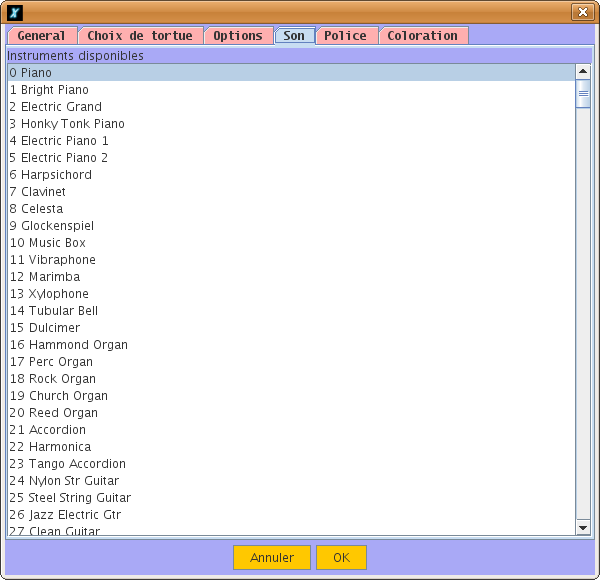
\includegraphics[scale=0.4]{images/CapturePref4.png}
	\end{center}
	\vspace{0.25cm}
	\item \textbf{Onglet Son}: vous trouverez la liste des instruments que peut imiter votre carte son au travers de l'interface MIDI. Vous pouvez sélectionner un instrument précis en cliquant dessus. (Vous pouvez également également sélectionner un instrument avec la primitive  \texttt{fixeinstrument numéro}. Si la liste des instruments n'apparait pas, voir la FAQ en fin de manuel à ce sujet.
	\begin{center}
 		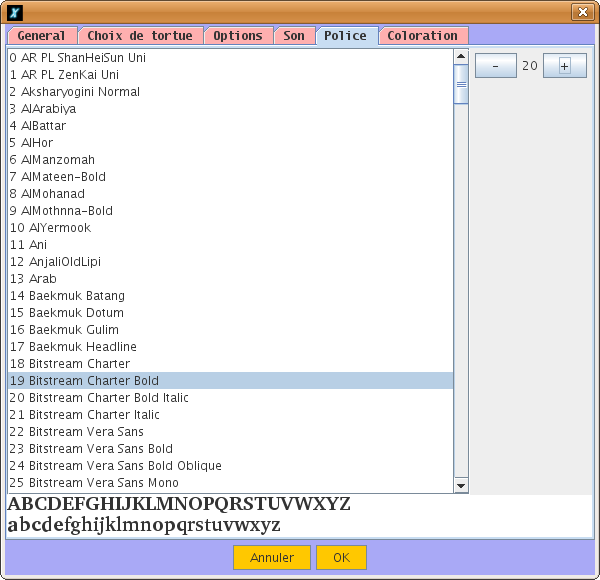
\includegraphics[scale=0.4]{images/CapturePref5.png}
	\end{center}
	\vspace{0.25cm}
	\item \textbf{Onglet Police}: Dans le cinquième onglet, vous pouvez choisir la police de l'interface graphique ainsi que sa taille. Attention ceci n'affecte pas la police rendue par les primitives \texttt{ecris} et \texttt{etiquette}.
	\begin{center}
 		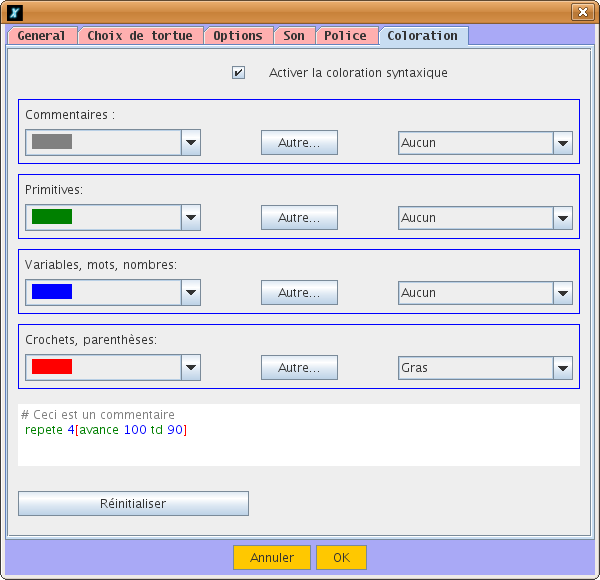
\includegraphics[scale=0.4]{images/CapturePref6.png}
	\end{center}
	\vspace{0.25cm}
	\item \textbf{Onglet Coloration syntaxique}: Possibilité d'activer ou non la coloration syntaxique et de définir des couleurs personnalisées.
\end{itemize}
\end{itemize}
\section{Menu \og Aide \fg}
\begin{itemize}
\item \textbf{Menu Aide$\to$Manuel en ligne}: Affiche le manuel de référence de \xlogo, accessible uniquement avec une connexion internet. 
	\vspace{0.25cm}
\item \textbf{Menu Aide$\to$Licence}: Affiche la licence GPL sous laquelle est distribué ce logiciel.
	\begin{center}
 		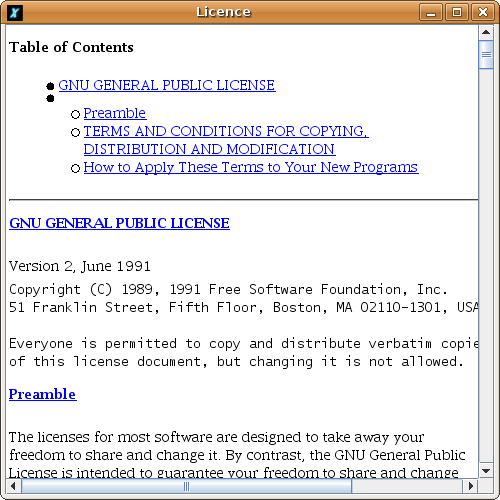
\includegraphics[scale=0.4]{images/CaptureLicence.png}
	\end{center}
	\vspace{0.25cm}
\item \textbf{Menu Aide$\to$Traduction française}: affiche une traduction de ladite licence. Cette traduction n'a aucune valeur officielle, seule la version anglaise
a ce rôle.

\item \textbf{Menu Aide$\to$Traduire XLogo}: Ouvre une boîte de dialogue permettant de consulter/modifier/compléter l'ensemble des traductions de XLogo (messages et primitives).\\
	\begin{center}
 		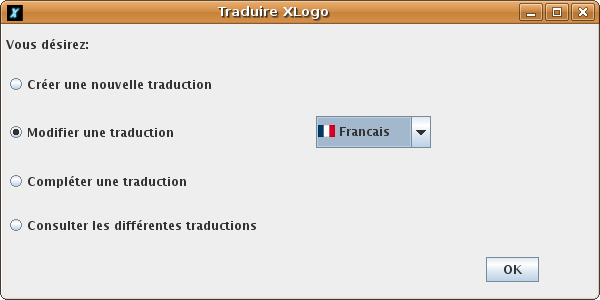
\includegraphics[scale=0.4]{images/CaptureXLogoTrad1.png}
 		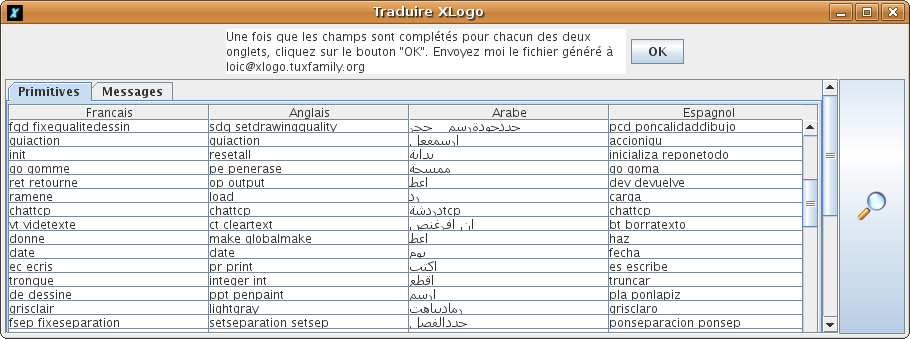
\includegraphics[scale=0.4]{images/CaptureXLogoTrad2.png}
	\end{center}
	\vspace{0.25cm}
 Il est également possible de créer les traductions pour une nouvelle langue. Dans chacun des cas le fichier généré est à envoyer à \texttt{loic@xlogo.tuxfamily.org}.\\
\item \textbf{Menu Aide$\to$A propos}: Classique .... et http://xlogo.tuxfamily.org pour vos mises à jours !! o:)\\
	\begin{center}
 		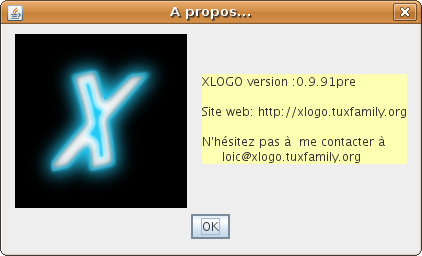
\includegraphics[scale=0.6]{images/CaptureApropos.png}
	\end{center}
	\vspace{0.25cm}
\end{itemize}


